\chapter{Implementation and Integration in Robots}
\label{chapt|implementation-integration}

\section{A centralized server-based implementation}
\label{sect|oro-server-impl}

The ORO server is a multi-platform command-line application that starts a
socket server to which clients can send requests to store or retrieve symbolic
statements.

Figure~\ref{fig|oro-impl} gives an overview of the ORO server architecture. The
server is build on three layers: a front-end, in charge of the communication
with external clients, a set of central modules that either handle incoming
requests or provide background processing (like the event monitoring or the
memory management), and a back-end, that stores the knowledge models in several
parallel pools of RDF triples, one per agent. The back-end provides all the
knowledge manipulation functionalitites required by the modules including
reasoning.

\begin{figure}
    \centering
    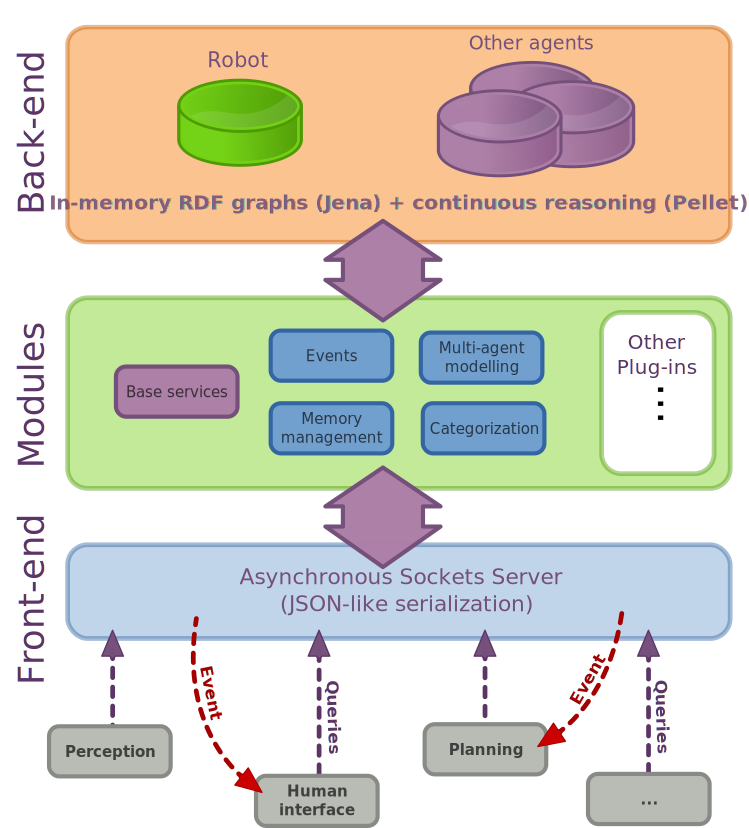
\includegraphics[width=0.7\columnwidth]{implementation/oro_impl.pdf}
    \caption{The software architecture of the ORO server.}
    \label{fig|oro-impl}
\end{figure}


The ORO server is written in Java 6. This choice is due to widespread use of
the Java language in the semantic Web community that leads to the fact that
most of the RDF/OWL API and reasoners are available as Java libraries. As
mentionned previously, the ORO server relies on the Jena API for OWL
manipulation and on the Pellet reasoner for all reasoning tasks. Java was thus
the best candidate to glue them in a robotic-friendly knowledge base.
Section~\ref{sect|java-impl} below gives more details on the Java
implementation of the server.

\subsection{Front-end}
\label{sect|frontend}

Communication with external components is handled by the server front-end.  It
was originally build as a YARP node, but was eventually transformed into a
simpler and more generic socket interface.  The socket connector uses a simple
ASCII protocol, presented in figure~\ref{fig|oro-protocol}.  Communication with
dedicated robotic middlewares like ROS or YARP is provided by dedicated
external clients. Section~\ref{sect|interfacing-middlewares} briefly presents
them.


\begin{SaveVerbatim}[frame=single, commandchars=\\\{\}]{PostPrtcl}
\emph{method}
\emph{[parameter1]}
\emph{[parameter2]}
\emph{[parameter n]}
#end#
\end{SaveVerbatim}

\begin{SaveVerbatim}[frame=single, commandchars=\\\{\}]{OkPrtcl}
ok
\emph{[return value]}
#end#
\end{SaveVerbatim}

\begin{SaveVerbatim}[frame=single, commandchars=\\\{\}]{ErrorPrtcl}
error
\emph{[exception name]}
\emph{[human-readable error]}
#end#
\end{SaveVerbatim}

\begin{SaveVerbatim}[frame=single, commandchars=\\\{\}]{EventPrtcl}
event
\emph{event id}
#end#
\end{SaveVerbatim}

\begin{figure}
\centering

\subfigure[Client requests]{
\BUseVerbatim{PostPrtcl}
} \\
\subfigure[Server answers]{
\BUseVerbatim{OkPrtcl}
\BUseVerbatim{ErrorPrtcl}
\BUseVerbatim{EventPrtcl}
}

\caption{The ORO server protocol. Elements in square brackets are optional.
Note that the {\tt ok} and {\tt error} message are synchronous server answers
to client requests while the {\tt event} message is produced asynchronously.}

\label{fig|oro-protocol}

\end{figure}

When a request is received by the front-end, it is parsed, deserialized and
dispatched to the module providing the requested service.

\subsection{Modules}

These \emph{modules} are initialized and maintained by the server. They provide
the actual features of the server as sets of \emph{services} (like \jmeth{add},
\jmeth{getSubclasses}, etc.).

Some modules do not expose any services. They provide instead other form of
knowledge management. For instance, the \jclass{MemoryModule} is in charge of
the application of the memory policies. It discards old statements depending on
the memory class they belong to (short term memory, long term memory, etc.).

Regular modules' services (that are actual Java methods) are invoked by the
front-end.  They process the request and interact with the knowledge pool via
the back-end interface.

\paragraph{Plugins} The server can be easily extended by the mean of
\emph{plugins}. These are JAR files that are loaded at run-time and have access
to the exact same internal APIs as regular modules like the event module or the
categorization module. The creation of new plugins is documented in a tutorial
available
on-line\footnote{\url{http://www.openrobots.org/wiki/oro-server-plugins}}.

\subsection{Back-end}
\label{sect|backend}

The back-end consists in a pair \emph{\{facts storage, reasonner\}}. For ORO,
we make the choice to rely the open-source {\sc Jena} library to store and
access the RDF graph, in combination with the {\sc Pellet} reasoner. However,
due to clean separation, other APIs (like the {\sc Manchester OWL-API} and
reasoners (like {\sc Fact++} or {\sc HermiT}) could be used with little changes
in the backend.

\subsubsection{Jena}
\label{sect|jena}

{\sc Jena}~\cite{McBride2002} is a mature library for the semantic Web,
originally developed by Helwett-Packard labs, and now under the leadership of
the Apache foundation.

As stated on its official website\footnote{{\sc Jena} website:
\url{http://incubator.apache.org/jena/}}, the Jena Framework includes:

\begin{itemize}
    \item an API for reading, processing and writing RDF data in XML, N-triples
    and Turtle formats;
    \item an ontology API for handling OWL and RDFS ontologies;
    \item a rule-based inference engine for reasoning with RDF and OWL data
    sources;
    \item stores to allow large numbers of RDF triples to be efficiently stored
    on disk;
    \item a query engine compliant with the latest SPARQL specification
    \item servers to allow RDF data to be published to other applications using
    a variety of protocols, including SPARQL
\end{itemize}

\subsubsection{Pellet}
\label{sect|pellet}

{\sc Pellet}~\cite{Sirin2007} is a reasoner for Description Logics developed by
Clark\&Parsia\footnote{{\sc Pellet} website:
\url{http://clarkparsia.com/pellet}}.

Pellet supports reasoning with the full expressivity of OWL-DL
($\mathcal{SHOIN(D)}$ in Description Logic jargon) and has been extended to
support the forthcoming OWL 2 specification ($\mathcal{SROIQ(D)}$).

Pellet provides all the standard inference services that are traditionally
provided by DL reasoners: consistency checking, concept satisfiability,
classification and realization (the most specific classes that an individual
belongs to). It also supports DL-safe SWRL rule.

\fxwarning{Rephrase this copy-paste from pellet website}

The use of a reasoner is completely transparent for the modules: the reasoner
is automatically called when a model changes and classifies it. Thus, queries
to the knowledge models always access both the \emph{asserted} and
\emph{inferred} sets of statements. As a consequence, the ORO server can be run
with no reasoner without any visible API change for the modules. They will
simply manipulate only asserted facts.

\subsubsection{API}

As of version 0.8, the ORO server API exposes about 50 methods (some of them
are besides polymorphic) organized into seven categories: \emph{Base}, \emph{Agents},
\emph{Administration}, \emph{Concept comparison}, \emph{Events}, \emph{Queries}
and \emph{Taxonomy walking}.

Partial support for the \emph{Knowledge API} (section~\ref{sect|kb-api}) has
been added to ORO server 0.8: the newly introduced {\tt revise} method that
takes a \emph{revision policy} as parameter is a versatile and generic
mechanism that deprecates {\it de-facto} several methods currently exposed by
the API. In future releases, the API could in consequence be shortened.

The current API is provided in appendix~\ref{chapt|oro-api}.

\subsubsection{Java Implementation}
\label{sect|java-impl}

The ORO server has been developed with modularity in mind, thus most of its
structure relies on clearly defined Java interfaces.
Figure~\ref{fig|oro-impl-java} presents the main ones.

\begin{figure}
    \centering
    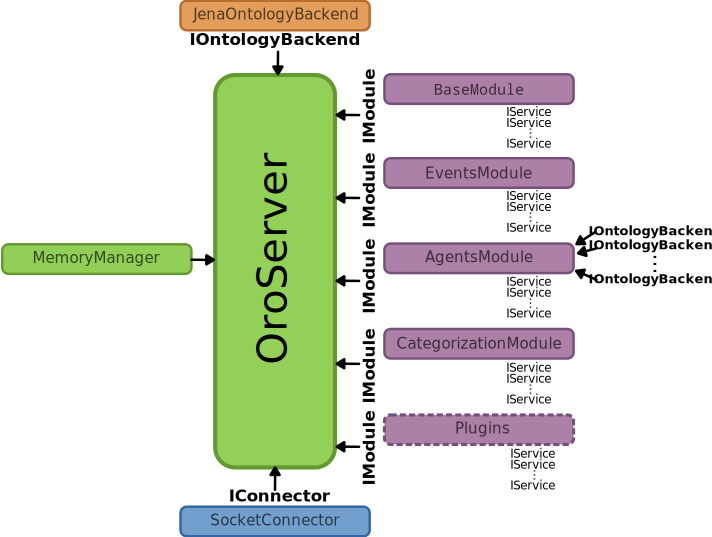
\includegraphics[width=0.9\columnwidth]{implementation/oro_impl_java.pdf}
    \caption{Main Java interfaces and classes of the ORO server.}
    \label{fig|oro-impl-java}
\end{figure}

The application entry point is the \jclass{OroServer} class. The class
instanciate one front-end (\jinterface{IConnector}), one main back-end
(\jinterface{IOntologyBackend}) and several modules (\jinterface{IModule}),
including plugins that are loaded at run-time.

Modules commonly also implement the \jinterface{IServiceProvider} interface to
expose \emph{services} (\jclass{IService}). These are the actual methods found
in the server API. Java methods that belongs to the API simply need to be
decorated with a \jinterface{@RPCMethod} Java annotation to automatically
exported. Extending the server API is thus simply a matter of annotating any
Java method with \jinterface{@RPCMethod}. Listing~\ref{code|oro-add} shows one
example of a service annotated in such a way, the {\tt add} method.

\lstset{language=java}
\begin{lstlisting}[caption=The {\tt add} method from ORO {\tt BaseModule}, 
                   label = code|oro-add, 
                   morekeywords={@RPCMethod}]
@RPCMethod(
        category="base",
        desc="adds one or several statements (triples S-P-O)."
)
public void add(Set<String> rawStmts, String memProfile)
{
    Set<IStatement> stmtsToAdd = new HashSet<IStatement>();
    
    for (String rawStmt : rawStmts) {
        if (rawStmt == null)
            throw new IllegalStatementException("Got a null stmt!");
        IStatement s = oro.createStatement(rawStmt);
        stmtsToAdd.add(s);
    }
    
    oro.add(stmtsToAdd, MemoryProfile.fromString(memProfile), false);
}
\end{lstlisting}


%%%%%%%%%%%%%%%%%
\section{Bindings to other components/languages}
\label{sect|interfacing}

To ensure the integration of ORO server in existing robotic architectures, we
have developed several idiomatic language-specific bindings, as well as bridges
with two widespread robotic middlewares, ROS and YARP.

\subsection{Language bindings}
\label{sect|bindings}

The main interaction gate with ORO server is its socket interface (as presented
above, at section~\ref{sect|frontend}). Sockets are light-weight, platform
independant, and supported by every programming languages.  Developing an
interface with ORO server in a new language is thus easy.

For our own needs, and because they are amongst the most widely used languages,
bindings for Python and C++ are available by default with ORO server.

The complete Python and C++ API will not be presented here (their
documentations are available on-line,
\footnote{\url{http://www.openrobots.org/wiki/oro-server-bindings}}), but we
present two short example that demonstrate how the knowledge base can be
integrated in code in a natural way.

\subsubsection{Python}
\label{sect|python-bindings}

The Python script below (listing~\ref{code|ex-python}) demonstrates several of
the interaction mechanisms with ORO server: model alteration, queries and events.

\lstset{language=python}
\begin{lstlisting}[numbers=left,
                   caption=Example of interaction with {\tt oro-server} in Python, 
                   label = code|ex-python,
                   morekeywords={as}]
import time
from pyoro import Oro, OroServerError

def onevent(evt):
        print("God save the queen! " + evt + " killed Bond!")

try:
        oro = Oro()

        oro += ["Spy rdfs:subClassOf Human", 
                "bond rdf:type Spy", 
                "bond rdfs:label \"Bond, James Bond\""]

        if "bond rdf:type Human" in oro:
            print("Alright, Bond is a human")

        oro += "pr2 rdf:type Robot"

        for ag in oro["* rdf:type Agent"]:
            print("Agent " + ag + " is here.")

        oro.subscribe(["?a kills bond"], onevent)
        oro += "pr2 kills bond"

        time.sleep(1)

except OroServerError as ose:
        print('Oups! An error occured!')
        print(ose)

finally:
        oro.close()
\end{lstlisting}

At line 8, we establish the connection to the server. We assume here that the
server is launched on the default port and on the local machine.

At line 10, three facts are added to the knowledge base. The first one modifies
the TBox of the ontology (alteration of the knowledge structure) while the two
other ones modify the ABox (a new instance and a new label). Adding (or
removing) triples from the ontology is done naturally with the {\tt +=} and
{\tt -=} operators.

At line 14, we check that a fact holds, either in the asserted model or in the
inferred model (in this case, Bond is inferred to be a human because we added
before that spies are types of humans). Here as well we use a natural idiomatic
Python syntax.

Line 19 shows how queries can be executed, with a dictionary-like accessor.
Both humans and robots are asserted to be agents in the ORO common-sense
ontology, thus this query returns a list {\tt [bond, pr2]}.

Line 22 shows how events are created. We first subscribe to an event by passing
a pattern ({\tt ?a kills bond}) and a callback (implemented at lines 4-5).
Line 23 triggers the event, and the callback method is then invoked.

We have kept this example simple. The complete Python API allows to describe
more complex events (when a fact can not be inferred, when a new instance of a
given class appears, etc.), to manipulate different models, to walk through the
ontology taxonomy, etc.

\subsubsection{C++}

The C++ bindings are provided as a library called {\tt liboro}. The
listing~\ref{code|ex-cpp} presents some examples of its usage.

\lstset{language=c++}
\begin{lstlisting}[numbers=left,caption=Example of interaction with {\tt oro-server} in C++, label = code|ex-cpp]
#include <iostream>
#include <iterator>
#include <set>

#include "liboro/oro.h"
#include "liboro/oro_library.h"
#include "liboro/socket_connector.h"

using namespace std;
using namespace oro;

class EventCallback : public OroEventObserver {
    void operator()(const OroEvent& evt) {
    cout << "Event triggered!" << endl;
    }
};
  
int main(void) {
  set<Concept> result;
  set<string> partial_stmts;
  
  SocketConnector connector("localhost", "6969");
  Ontology *oro = Ontology::createWithConnector(connector);
  
  //Creation of instances
  Agent robot1 = Agent::create("Nice Robot", Classes::Robot);
  Agent human = Agent::create("Young PhD", Classes::Human);
  
  //First query
  partial_stmts.insert("?mysterious rdf:type Agent");
  oro->find("mysterious", partial_stmts, result);
  
  copy(result.begin(), 
       result.end(), 
       ostream_iterator<Concept>(cout, "\n"));
  
  partial_stmts.clear();
  result.clear();
  
  //More statements are added to the knowledge base
  Object table = Object::create(Classes::Table);

  Object unknown_object = Object::create();
  unknown_object.assertThat(Properties::isOnTopOf, table);
  
  oro->add(Statement("oro:isOnTopOf rdfs:subClassOf oro:isAt"));
  
  Agent myself("myself");
  
  myself.sees(unknown_object);
  myself.sees(human);
  
  //A query involving multiple partial statements
  partial_stmts.insert("?mysterious isAt ?support");
  partial_stmts.insert("?support rdf:type cyc:Table");
  partial_stmts.insert("oro:myself sees ?mysterious");
  
  oro->find("mysterious", partial_stmts, result);
  
  copy(result.begin(), 
       result.end(), 
       ostream_iterator<Concept>(cout, "\n"));
  
  //Events
  EventCallback ec;
  Classes::Human.onNewInstance(ec);
  Agent superman = Agent::create("Superman", Classes::Human);
  
  sleep(1);
  
  set<string> event_pattern;
  Property flyingProp = Property("isFlying");
  
  event_pattern.insert( superman.id() + " isFlying true");
  oro->registerEvent(ec, 
                     FACT_CHECKING, 
                     ON_TRUE_ONE_SHOT, 
                     event_pattern, "");
  
  superman.assertThat(flyingProp, "true");
  
  sleep(1);
  
  return 0;
}

\end{lstlisting}

At lines 22 and 23, the {\tt oro} object is built as a singleton. This
actually connects the application to the ontology server.

At line 26 and 27, we create two new instances of agents labeled \emph{Nice
Robot} and \emph{Young PhD} (the static types {\tt Classes::Robot} and {\tt
Classes::Human} are generated from the ontology itself by a script).

A first, simple query (line 30 and 31) return a {\tt std::set} of concept IDs.

At line 41, a new object is created. No label is defined, but the
class is set to be a table. On the contrary, at line 43, we create a generic
object (only asserting it is an instance of {\tt Object}).

At line 44, we assert a property (here also, the list of available properties is
statically generated from the ORO ontology).

As shown at line 46, we can as well access the ontology at a lower level,
directly adding (or removing) new triples. In this case, we modify the TBox of
the knowledge base.

C++ objects can also be created by using directly the concept IDs, as shown
line 48 for the special concept {\tt myself} (an instance always representing
the robot itself). Some object properties frequently used in the ontology are
available as methods, as seen lines 50 and 51.

Lines 54 to 58 show a more complex query, involving several partial statements.
Named variables (like {\tt ?mysterious} or {\tt support}) are used in the
statements to reference the same entity.

Lastly, lines 65 to 80 show two ways of defining events with a callback functor
(defined at lines 12-16).

To deal with real-world constraints, {\tt liboro} also provides mechanisms to
reconnect to the ontology server when the connection is lost, and has a
built-in buffering system to increase bandwidth for components that produce a
large amount of symbolic facts.

\subsection{Interface with robotic middlewares}
\label{sect|interfacing-middlewares}

While convenient in certain cases, language-level interfaces do not usually
offer the modularity and loose-coupling required by complex robotic
architectures where tenth of modules, possibly spread over several CPUs, need
to talk together. The acknowledgement of this issue has led to the development
over the last ten years of numerous so-called \emph{robotic middlewares} that
abstract away inter-module communication (at the transports, protocols and
programming interfaces levels).

We provide with ORO server wrappers for two of the main middlewares currently
in use in the robotic community, ROS~\cite{Quigley2009} and
YARP~\cite{Metta2006}.

These wrappers use the C++ or Python bindings previously presented to expose
the functionalities of ORO server as a stand-alone ROS/YARP nodes.

%%%%%%%%%%%%%%%%%
\section{Monitoring and debugging}
\label{sect|monitoring}

\subsection{Logging}

The ORO server offers several levels of logging, from ``almost silent'' to very
verbose. In verbose mode ({\tt debug} level), the server outputs exact incoming
requests, along with millisecond accurate timestamps.

Those logs can then be replayed by a special tool written in Python that
simulates the original communication with the server: timestamps are respected
and if multiple clients where connected to the server, the log player forks one
thread by client to simulate parallel access to the server.

\subsection{Visualisation}

\begin{figure}
    \centering
    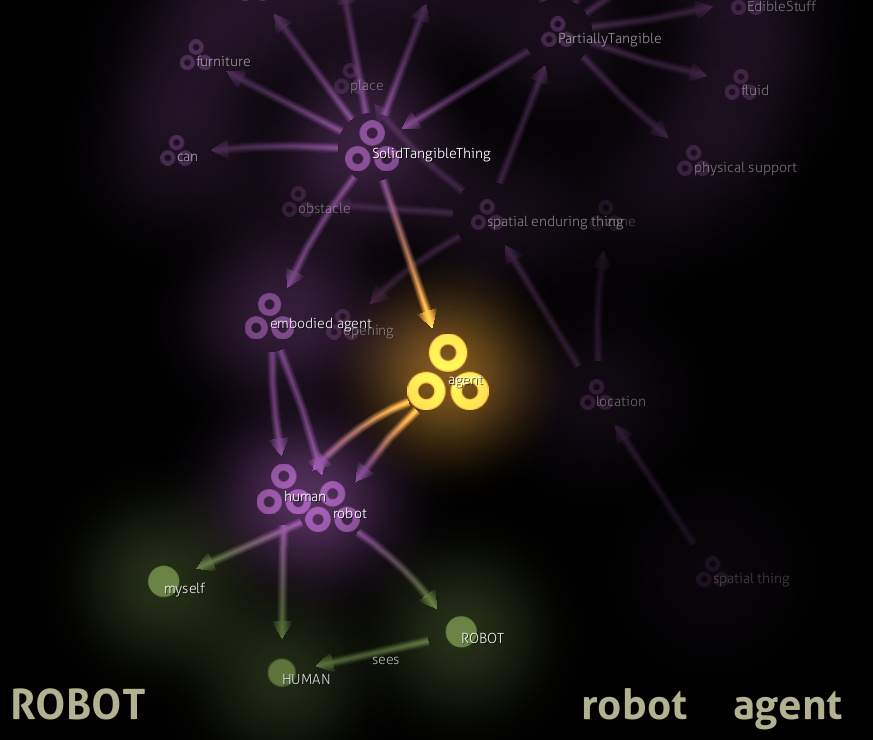
\includegraphics[width=0.7\columnwidth]{implementation/oroview.jpg}
    \caption{A screenshot of the {\tt oro-view} visualisation tool.}
    \label{fig|oroview}
\end{figure}

Visualisation of ontologies is a difficult task in general because of their
complex graph structure. In order to present anyway the content of the ontology
to external observers, we have developed an OpenGL-based dynamic visualiser
called {\tt oro-view} (figure~\ref{fig|oroview}). This application connects to
the ORO server and lets the user explore the taxonomy by simply selecting
concepts on the screen. Nodes are expanded, distributed in a force-oriented
graph, and further reveal the structure of the ontology. Because {\tt oro-view}
takes on-demand its input from the server, changes in the ontology (new facts
being added, etc.) are reflected in the viewer when the user refreshes nodes.

{\tt oro-view} also subscribes at startup to a special event for \emph{active
concepts} (\ie it monitors ne instances of the \concept{ActiveConcept} class).
Each time an individual is asserted to be an \concept{ActiveConcept}, the
server triggers back {\tt oro-view} that creates a visual focus on the concept
(the individual ``pops up''). When displayed during experiments, this provides
nice-looking visual feedback to external observers. In particular, we made use
of this feedback during the public performance of the \emph{Roboscopie} theatre
play (section~\ref{sect|roboscopie}).

{\tt oro-view} also provides export to GraphViz {\tt dot} format for latter
reuse of the ontology graph in publications.

%%%%%%%%%%%%%%%%%
\section{Integration in the robot architecture}

\begin{figure*}[thpb]
  \centering
  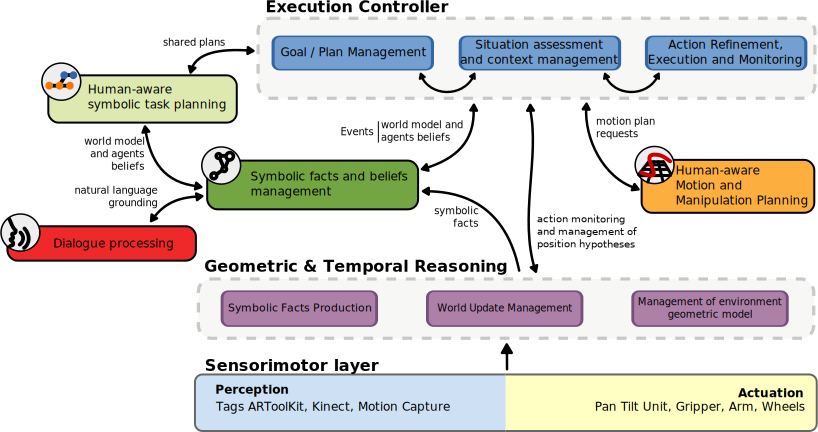
\includegraphics[width=0.9\columnwidth]{integration/architecture_overview.pdf}
  \caption {Software architecture for a service robot interacting with humans.}
  \label{fig|archi}
\end{figure*}

Figure~\ref{fig|archi} presents the organization of the ``cognitive'' layer of
the service robots Jido and PR2 as currently in service at LAAS (this
architecture is described in detail in~\cite{Alami2011}). The sensorimotor
layer (bottom) is abstracted in SPARK, an intermediate amodal 3D model where
geometric (and some temporal) reasoning take place~\cite{Sisbot2011}.

The outcome of the geometric analysis, as well as the result of the dialogue
processing module ({\sc Dialogs}, are stored in ORO, that acts as a central
knowledge base. The symbolic knowledge base triggers events that are captured
by a top-level execution controller (for instance, SHARY~\cite{Warnier2012}).

The controller can rely on two specialized planners: MHP, the geometric motion
and manipulation planner~\cite{Sisbot2008, Mainprice2011, Pandey2010} and HATP,
the symbolic task planner~\cite{Alili2008}.

The dialogue processing module, as well as the symbolic task planner, also use
the knowledge base to answer questions or initialize the planning domain.

During a typical interaction experiment, the execution controller decides upon
a plan to execute, requires a plan from the task planner, allocates the actions
to the human and the robot, communicates the shared plan, and controls and
monitors its execution. The operation continues until the goal is achieved, is
declared unachievable or is abandoned by the human.

Only ORO and Dialogs, as components, are actual direct outcomes of this
doctoral work. It is however important to present them all here since a
knowledge base only make sense within a larger architecture, with knowledge
providers and consumers.  Furthermore, the approach to knowledge management
introduced by this thesis had a strong influence on the design of the
communication flows between all these components. Thus, this section introduces
the software components that have been used in conjunction with ORO (mostly,
but not only, on the LAAS robots), and details how these components produce,
exchange and consume symbolic knowledge.

\subsection{RPC and events-oriented interactions}

\subsection{Acquiring and Anchoring Knowledge in the physical world: the SPARK module}

\subsubsection{Building an Agent-Aware Symbolic Model of the Environment}
\label{sect|situ}

Anchoring perceptions in a symbolic model requires perception abilities and
their symbolic interpretation. In this section we present SPARK (\emph{SPAtial
Reasoning \& Knowledge}~\cite{Sisbot2011}), a situation assessment reasoner
that generates relevant symbolic information from the geometry of the
environment with respect to relations between objects, robots and humans.

\begin{figure}[ht!]
   \begin{center}
%
       \subfigure{
           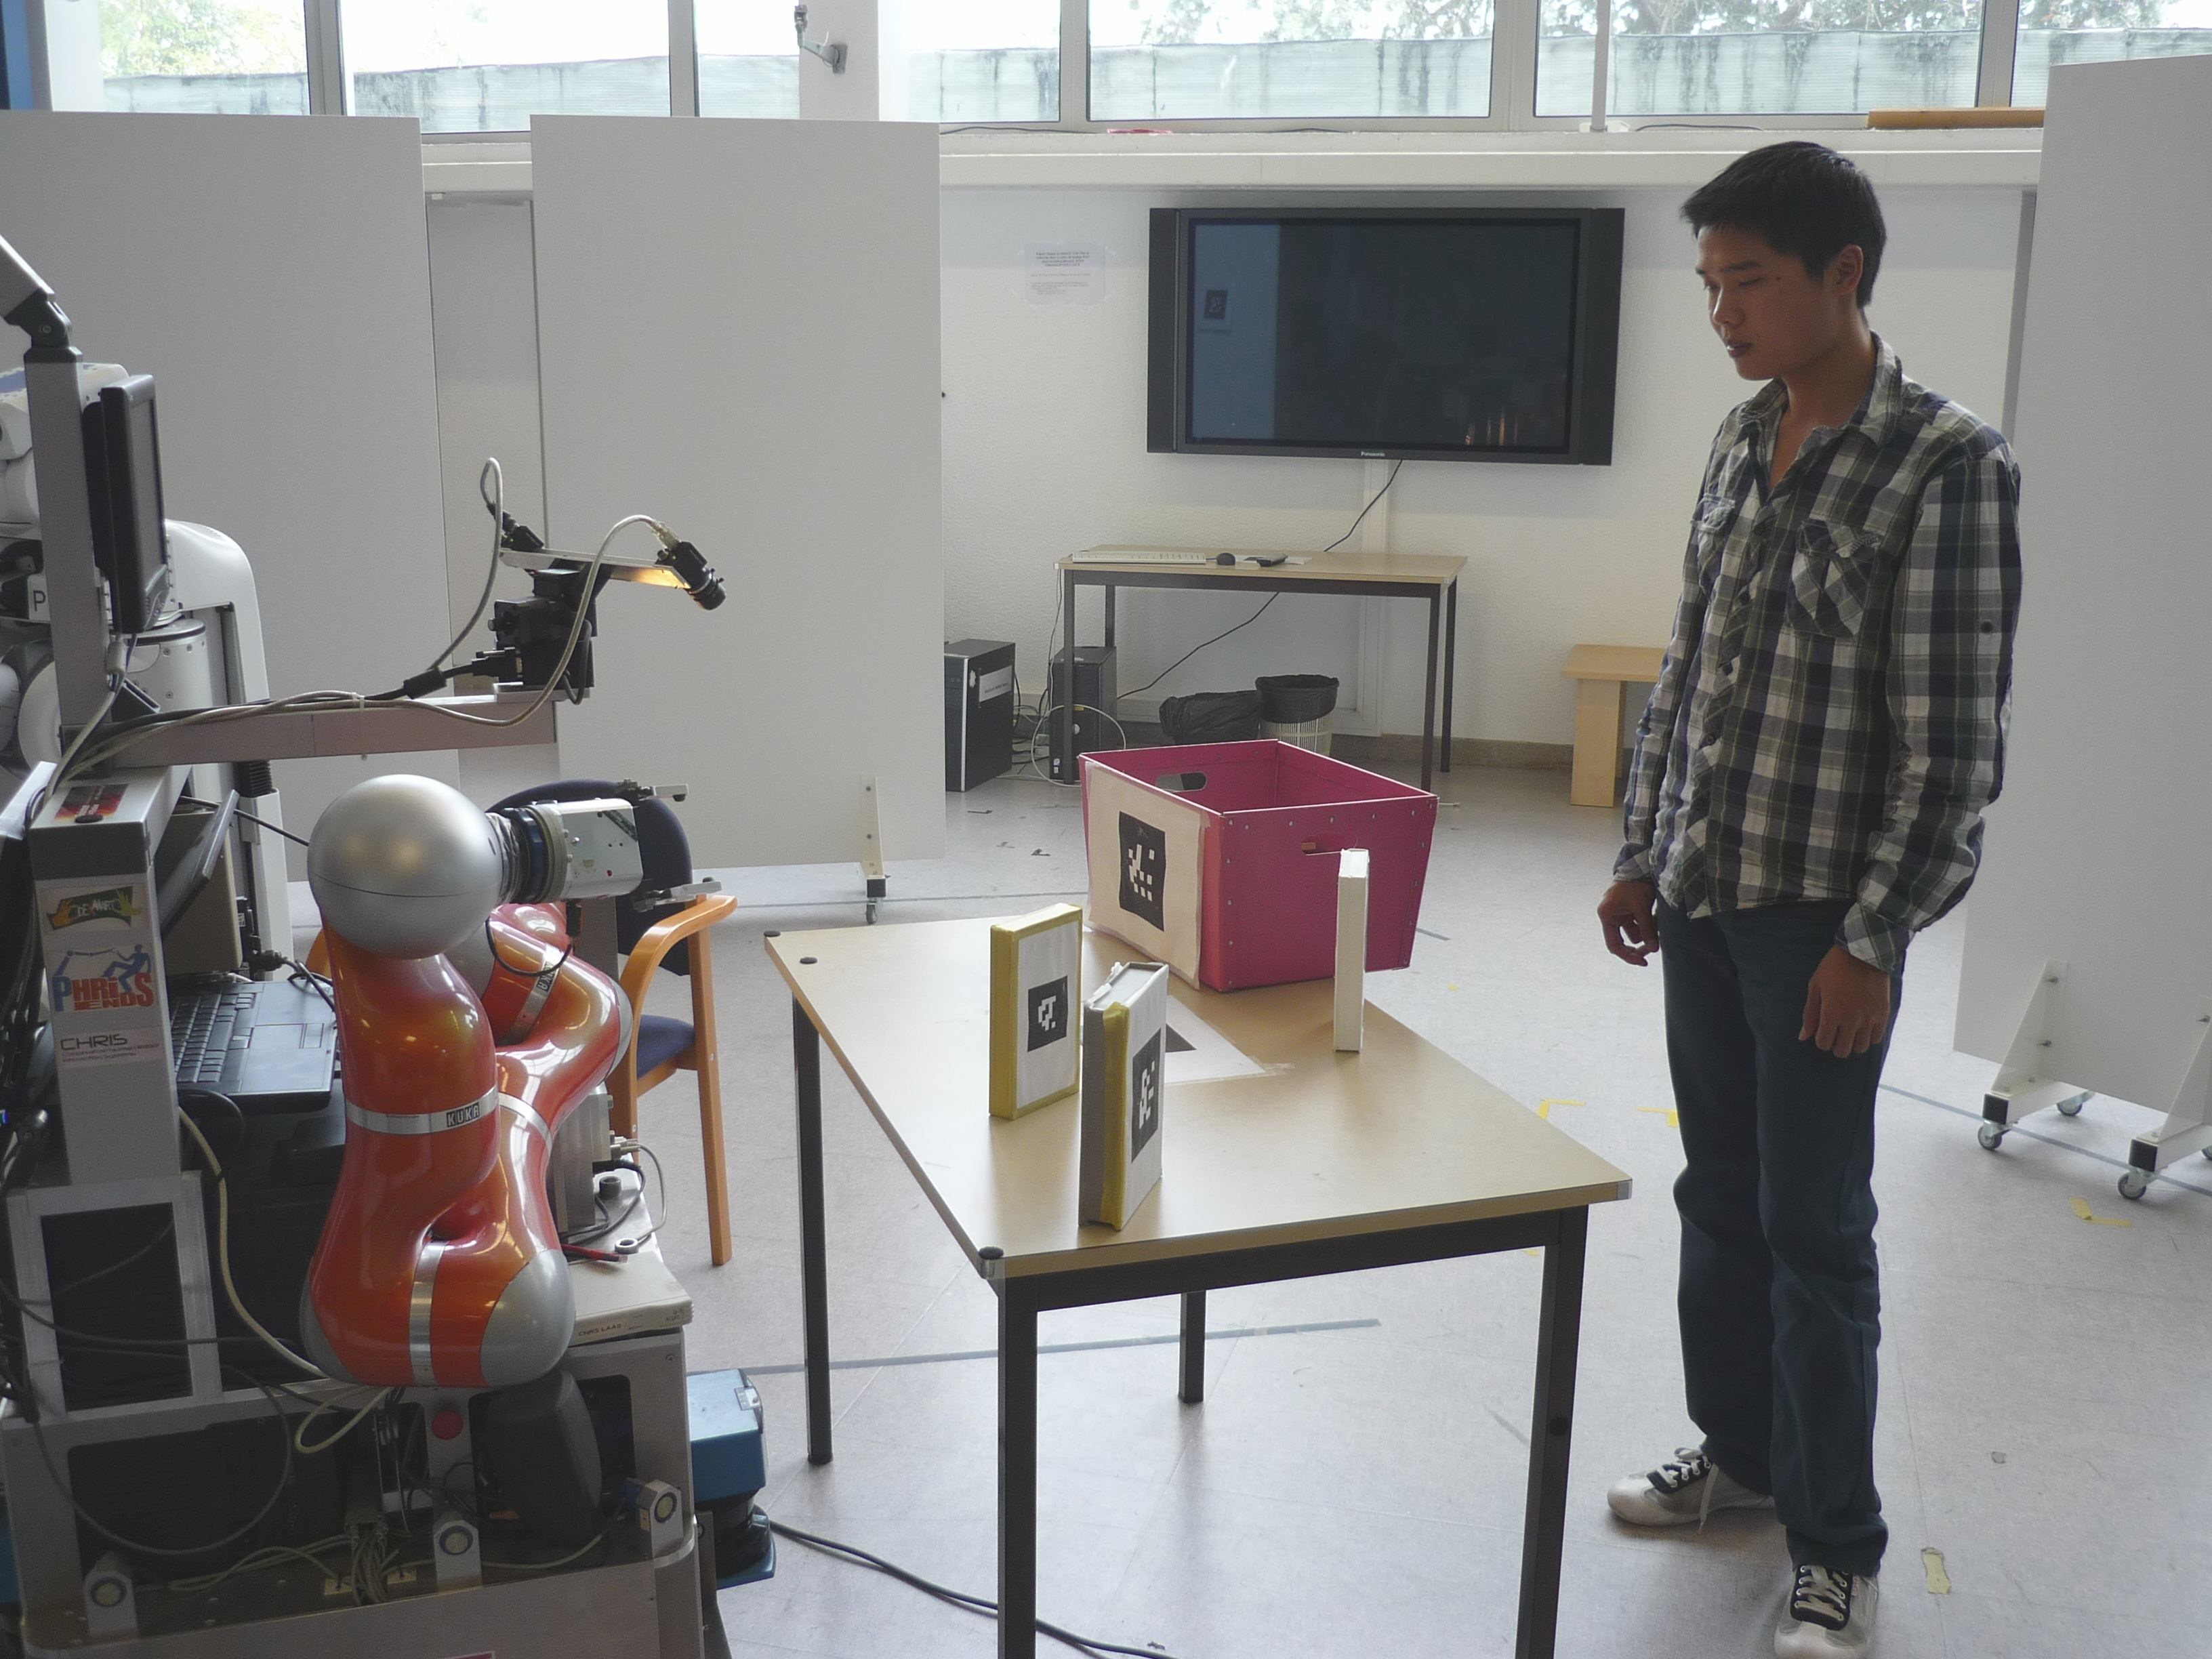
\includegraphics[width=0.5\textwidth]{spark/etat.jpg}
       }%
       \subfigure{%
          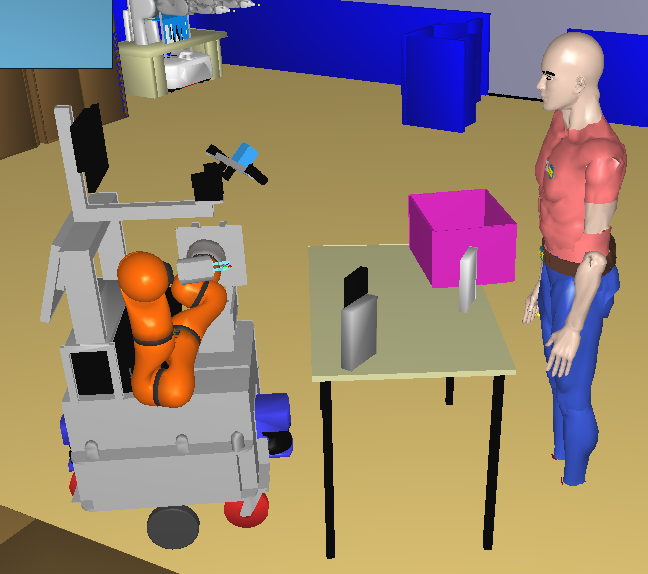
\includegraphics[width=0.43\textwidth]{spark/etat_spark.png}
       }\\ %  ------- End of the first row ----------------------%
%
   \end{center}

   \caption{The robot represents at runtime its environment in a 3D model
   resulting of the sensors' inputs fusion (Kinect, motion capture, 2D barcodes
   tracking).}

   \label{fig|spark}

\end{figure}

Figure~\ref{fig|spark} shows a screenshot of the SPARK environment side-by-side
with the real environment: as mentioned in the introduction, objects are
identified and localized through 2D barcodes. The human pose is tracked with
a Microsoft Kinect device (assisted by motion capture to accurately track the
head motion, which is required to compute what the human is looking at).

This geometric model is continuously updated at runtime by the robot.

\paragraph{Symbolic locations}

Human commonly refer to the positions of objects with symbolic descriptors
(like \emph{on}, \emph{next to}...) instead of precise, numeric position. These
type of descriptors have been studied in the context of language grounding
(\cite{O'Keefe1999,Matuszek2010,Regier2001,Kelleher2006,Blisard2005}). In this
work we focus agent-independent symbolic locations and agent-dependent,
relative locations.

\paragraph{Agent-independent locations}

We can refer to object locations with respect to other objects in the
environment, such as \emph{above, next to, in}, etc. In this work we compute
three main relations based on the bounding box and center of mass of the
objects (fig.~\ref{fig|sprelations}): 

\begin{itemize}
	\item \concept{isOn}: computes if an object $O_1$ is on another object $O_2$ by
	evaluating the center of mass of $O_1$ according to the bounding box of $O_2$.

	\item \concept{isIn}: evaluates if an object $O_1$ is inside another object
	$O_2$ based on their bounding boxes $BB_{O_1}$ and $BB_{O_2}$.

	\item \concept{isNextTo}: indicates whether an object $O_1$ is next to another
	object $O_2$. We cannot use a simple distance threshold to determine if two
	objects are next to each other since the relation is highly dependent on the
	dimensions of the objects. For instance, the maximum distance between large
	objects (\eg two houses) to consider them as being next to each other is much
	larger than the maximum distance we would consider for two small objects (\eg
	two bottles). Thus, the relation between the dimensions and the distances of
	the objects are taken into account.  

\begin{figure} 
	\centering
	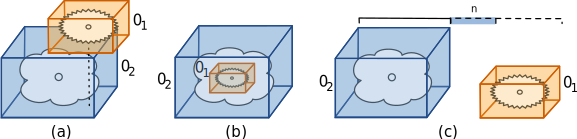
\includegraphics[width=0.95\columnwidth]{spark/spatial_relation.pdf}
	\caption{Spatial relations between two objects: (a) \concept{isOn} relation, 
	(b) \concept{isIn} relation, and (c) \concept{isNextTo} relation.} 
	\label{fig|sprelations} 
\end{figure}

\end{itemize} 

To ensure the different agent models are up-to-date, all these properties are
always computed on-line, each time the current state of the world changes.

Table~\ref{facts|sprelations} lists all the symbolic relationships that are
currently computed by the system.

\begin{table}[h]
    \centering
    \begin{tabular}{p{1.5cm}p{5cm}p{2cm}p{2.7cm}}
	\rowcolor{white}
    \textbf{Subject} & \textbf{Predicate} & \textbf{Object} & \emph{Notes} \\ 
    \hline
	 \concept{Location} & \concept{isAt} $\equiv$ \concept{cyc:objectFoundInLocation}  &  \concept{Location} & \\ 
	 &  $\rightarrow$ \concept{isOn} $\equiv$ \concept{cyc:above\_Touching}  &  & \\ 
	 &  $\rightarrow$ \concept{isIn}  &  & \\ 
	 &  $\rightarrow$ \concept{isNextTo}  & &  \\ 
	 \concept{Location}  & \concept{isAbove} $\equiv$ \concept{cyc:above-Generally}  &  \concept{Location}  &  inverse of \concept{isBelow} \par \concept{isOn} $\Rightarrow$ \concept{isAbove}\\ 
	 \concept{Location}  & \concept{isBelow}  & \concept{Location}  &  inverse of \concept{isAbove}
	\end{tabular}

	\caption{List of statements describing spatial relationships between
	objects. ``$\rightarrow$'' indicates sub-properties. When existing, the
	equivalent predicate in the {\sc OpenCyc} standard (prefix \concept{cyc:})
	has been added.}

\label{facts|sprelations}
\end{table}

SPARK also compute symbolic facts related to agent independent world dynamics.
The predicate \concept{isMoving} states, for each tracked entity, whether it is
currently moving or not.


\paragraph{Agent-dependent placements}

While in previous section we listed several \emph{absolute} location predicate,
many topological relations are directly dependent from the observation point.

The predicate \concept{hasRelativePosition} represents spatial locations
between agents and objects that are agent dependent.  For example we say ``it
is on my right, on your left, ...'' We compute these spatial locations by
dividing the space around the referent (an agent) into $n$ regions based on
arbitrary angle values relative to the referent orientation.  For example, for
$n = 4$ we would have the space divided into \emph{front, left, right} and
\emph{back}. Additionally, two proximity values, \emph{near} and \emph{far},
may also be considered. The number of regions and proximity values can be
chosen depending on the context where the interaction takes place.


To build an agent-dependent model of the world, \emph{Perspective
Taking}~\cite{Flavell1992,Tversky1999} is employed by the reasoner to provide
the robot with the ability to put itself at the human's place (by moving a
camera in the geometric model) and to reason about the world from different
perspectives.


Through perspective taking, SPARK computes for each agent a symbolic
description of the relative positioning of objects in the environment (table
\ref{facts|relative}).

\begin{table}[h]
	\centering
	    \begin{tabular}{p{1.5cm}p{6cm}p{1.5cm}l}
		\rowcolor{white}
		\textbf{Subject} & \textbf{Predicate} & \textbf{Object} & \emph{Notes} \\
		\hline
	 \concept{Location}  & \concept{hasRelativePosition}  & \concept{Location} & \\ 
	 & 	$\rightarrow$ \concept{behind} $\equiv$ \concept{cyc:behind-Generally}  &  & inverse of \concept{inFrontOf}  \\ 
	 &  $\rightarrow$ \concept{inFrontOf} $\equiv$ \concept{cyc:inFrontOf-Generally}  & 	 & 	 inverse of \concept{behind}  \\ 
	 &  $\rightarrow$ \concept{leftOf}  &  &  inverse of \concept{rightOf} \\ 
	 &  $\rightarrow$ \concept{rightOf}  & 	 & 	 inverse of \concept{leftOf}  \\ 
	 \concept{Object}  & \concept{cyc:farFrom}  &  \concept{Agent} & \\ 
	 \concept{Object}  & \concept{cyc:near}  &  \concept{Agent} & 
	\end{tabular}
	\caption{List of statements describing relative spatial relationships between objects and agents.}
	\label{facts|relative}
\end{table}


\subsubsection{Building a Model of Agents}
\label{sect|grounding_agents}

Building a grounded symbolic model of the physical environment does not suffice
in general to fully ground the human-robot interaction.

We divide the process of building models for agents into two categories:
operations related to the assessment of the current situation (for instance,
\emph{What does the human do? What does he see?}), and operations related to
the estimation of potential actions (for instance, \emph{Which regions could
the human reach if I want to hand over an object?}). We call these
potentialities of action \emph{Mightabilities}.

\paragraph{Agent Capabilities}

There are a number of common properties for a robot and a human related to
their capabilities in a given situation: they can both reach, grasp, look at,
point at, etc.: we group them in the \emph{Agent} category, defined as entities
that can act in the environment and manipulate it.

In this work we focus on the following capabilities from each agent's
perspective:

\begin{itemize}

\item \emph{Sees}: An important ability to know about an agent is to predict
\emph{What can it see?}, \ie what is within its field of view (FOV). A robot being
able to compute this information can then act accordingly. An example would be
a clarification scenario where the human is searching for an object and the
robot is able to infer that he/she is looking for the one that is not visible
(otherwise the user would not be searching for it).  In
Figure~\ref{fig::sparkRepresentations}\emph{a} the field of view of a person is
illustrated with a grey cone (broader one). While he is able to see the two
small boxes on the table in front of him, the big box on his right is out of
his FOV, and therefore, he is not able to see it. 

\item \emph{Looks At}: this relation corresponds to what the agent is focused
on, \ie where its focus of attention is directed. This model is based on a
narrower field of view, the field of attention (FOA). 
Figure~\ref{fig::sparkRepresentations}\emph{a}
shows the field of attention of a person with a green cone (narrower one). In
this example only the grey box satisfies the \concept{looksAt} relation.

\item \emph{Points At}: verifies whether an object is pointed at by an agent.
This relation is particularly useful during interaction when one of the agents
is referring to an object saying ``this" or ``that" while pointing at it.
 
If a larger object occludes a smaller one while an agent is pointing at them, the
outcome of the evaluation will result only in one relation, \ie \stmt{agent\_01
pointsAt object\_01} since the small one is not visible to the agent.  On the
contrary, if the small object is in front of the big one, then both objects
will satisfy the relation, which may generate an ambiguity (which object the
agent refers to?) that should be solved through higher level reasoning (\eg
context analysis or clarification through verbal interaction).

\item \emph{Reachable}: it allows the robot to estimate the agent's capability
to reach an object, which is fundamental for task planning. For example, if the
user asks the robot to give him/her an object, the robot must compute a transfer
point where the user is able to get the object afterward. 
Figure~\ref{fig::sparkRepresentations}\emph{b} shows different reachability postures for each object
on the table. In the example, the bottle and the box are both reachable for the
human, but the teddy bear is too far. Instead, from the robot's perspective,
the teddy bear is reachable, while the bottle is not.

\end{itemize}

\begin{figure*}[!t]
	\begin{center}
	\subfigure[]{
		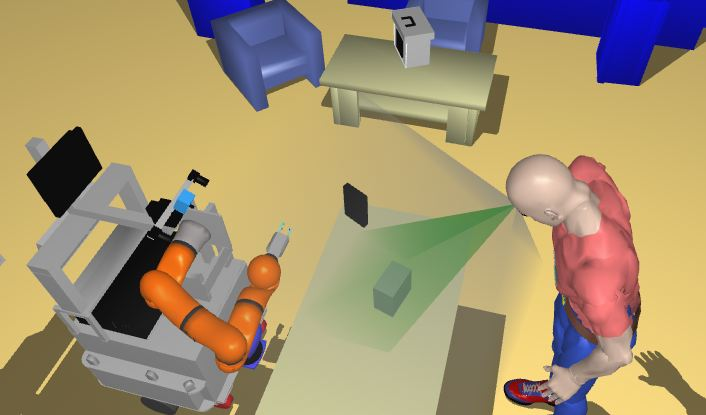
\includegraphics[width=0.4\linewidth]{spark/looks.jpg} 
	}
	\subfigure[]{
		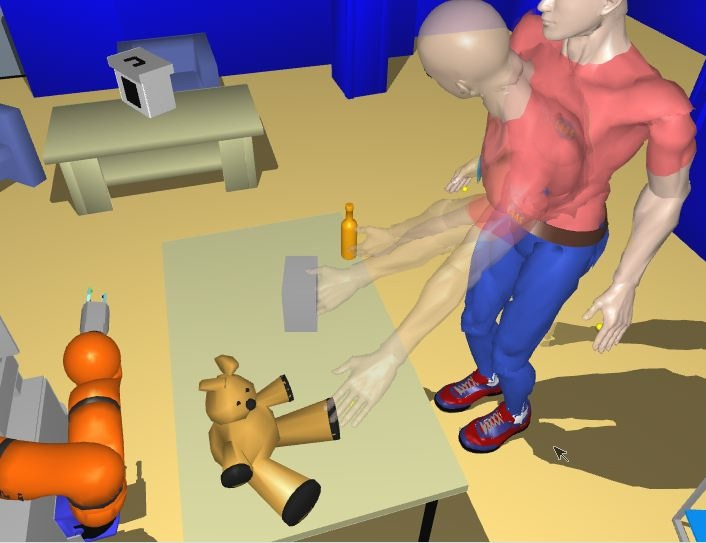
\includegraphics[width=0.35\linewidth]{spark/reach.jpg}
	} 
	\caption{(a) Field of view (FOV) and the field of attention (FOA) of the human. (b) Different reaching postures for the human.}
	\label{fig::sparkRepresentations}
	\end{center}
\end{figure*} 


While the first three relations (\concept{sees}, \concept{looksAt} and
\concept{pointsAt}) are computed through a model based approach, the latter one
is based on the Generalized Inverse Kinematics with pseudo inverse
method~\cite{Nakamura90,Baerlocher04} to find a posture for the
agent where its end-effector is at the center of the object within a given
tolerance.

Tables~\ref{facts|capabilites} summarizes the predicates produced by SPARK
during the agent capabilities analysis phase.

\begin{table}[h]
	\centering
		\begin{tabular}{p{2cm}p{4.5cm}p{2cm}p{3.5cm}}
		\rowcolor{white}
		\textbf{Subject} & \textbf{Predicate} & \textbf{Object} & \emph{Notes} \\
		\hline
		 \concept{Agent}  & \concept{looksAt}  & \concept{SpatialThing} \\
		 \concept{Agent}  & \concept{sees}  &  \concept{SpatialThing}  &    \\ 
		 \concept{SpatialThing}  & \concept{isInFieldOfView}  &  \concept{xsd:boolean}  & via inference: \par \stmt{myself sees *} $\Leftrightarrow$ \stmt{* isInFieldOfView true} \\ 
		 \concept{Agent}  & \concept{pointsAt} $\equiv$ \concept{cyc:pointingToward}  & \concept{SpatialThing} \\ 
		 \concept{Agent}  & \concept{focusesOn}  &  \concept{SpatialThing}  &  via inference: \par \concept{looksAt} $\wedge$ \concept{pointsAt} $\Rightarrow$ \concept{focusesOn} \\
		\concept{Agent} & \concept{seesWithHeadMovement} &  \concept{SpatialThing} \\
		\concept{Agent} & \concept{reaches} &  \concept{Object} \\ 

	\end{tabular}

	\caption{List of facts describing the attentional state and the abilities
	of an agent. \concept{looksAt} is interpreted as an object \emph{being in
	the field of attention} of an agent. An object is \concept{see}n if it is
	visible for the agent without moving the head (\ie, in \emph{field of
	view}).}

	\label{facts|capabilites}
\end{table}

Table~\ref{facts|agentstate} lists the other symbolic facts that are
produced and maintained by SPARK related to the general state of the agent.

\begin{table}[h]
	\centering
	\begin{tabular}{p{2cm}p{5cm}p{2cm}}
		\textbf{Subject} & \textbf{Predicate} & \textbf{Object} \\
		\hline
		\concept{Agent} & \concept{hasIn\{Left|Right\}Hand}  &  \concept{GraspableObject} \\ 
		\concept{Agent} & \concept{hasPosture}  &  \concept{Posture} \\
		\concept{Agent} & \concept{currentlyBodilyDoes}  &  \concept{Action}
	\end{tabular}

	\caption{List of statements describing the state of an agent in general.
	\concept{Posture} can be either \concept{standing} or \concept{sitting}.
	The \concept{currentlyBodilyDoes} predicate states the current action of
	the agent, be it intentional or not.}

	\label{facts|agentstate}
\end{table}

%%%%%%%%%%%%%%%%%

\subsection{Symbolic Task Planning}

Complex human robot interaction may necessitate a strong reasoning about the
environment and the capabilities of involved agents: How can they achieve a
specific goal? What are the required actions to achieve this goal? Which
actions can be performed by each agent? etc.

In the previous sections, we have seen how symbolic knowledge is produced and
stored from the real physical world. In this section, we present one possible
way to use these symbolic models of the environment and interacting agents to
produce a plan of actions for a complex goal.

\begin{figure}
    \centering
    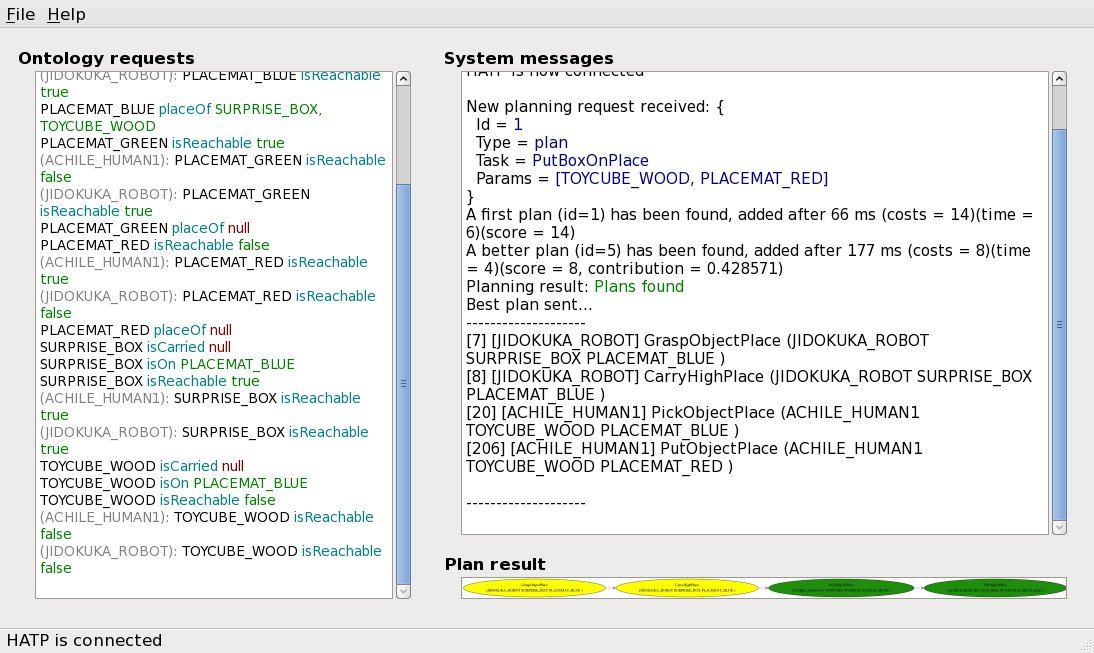
\includegraphics[width=0.9\columnwidth]{integration/hatp_console.jpg}
    \caption{Screenshot of the HATP console. On the left panel, we see the
    results of the requests to ORO, on the bottom right the resulting plan.}
    \label{fig|hatp_console}
\end{figure}

In order to devise how a given goal can be accomplished, the robot has to
elaborate a plan,\ie a set of actions to be achieved by the robot and its human
partners.  This is the role of HATP \cite{Alili2008} (for Human Aware Task
Planner, figure~\ref{fig|hatp_console}).  HATP is based on a Hierarchical Task
Network (HTN) refinement, which performs an iterative task decomposition into
sub-tasks until reaching atomic actions~\cite{Nau2003}.  The planning domain
defines a set of methods describing how to decompose a task and can be seen as
the {\it how-to} knowledge of the robot.  HATP is able to produce plans for the
robot's actions as well as for the other participants (humans or robots). It
can be tuned by setting up different costs depending on the actions to apply
and by taking into account a set of constraints called social rules. This
tuning aims at adapting the robot's behavior according to the desired level of
cooperation of the robot.

\paragraph{Agents and action streams} The robot plans not only for itself but
also for the other agents. The resulting plan, called ``shared plan'' is a set
of actions that form a stream for each agent involved in the goal achievement.
Depending on the context, some ``shared plans'' contain causal relations
between the agents. For example, the second agent needs to wait for the success
of the first agent's action to be able to start its own action. When the plan
is performed, causal links induce synchronization between agents.
Figure~\ref{plan_hatp1} illustrates a plan with two streams.

\begin{figure}[htbp]
  \centering
  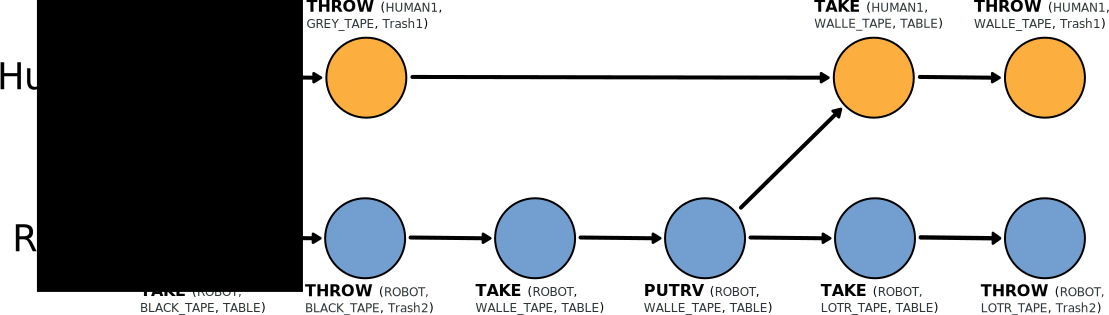
\includegraphics[width=0.8\columnwidth]{integration/hatp_plan1.pdf}
  \caption{A plan produced by HATP with 2 streams}
  \label{plan_hatp1}
\end{figure}

\paragraph{Action costs and social rules} A cost and a duration function is
associated to each action.  The duration function provides a duration interval
for the action achievement and is used, in one hand, to schedule the different
streams and, in the other hand, as an additional cost function.  In addition to
these costs, HATP also takes into account a set of social rules.  Social rules
are constraints aiming at leading the plan construction towards the best plan
according to some human preferences. The social rules we have defined so far
deal with:

\begin{itemize}

    \item undesirable state: to avoid a state in which the human could feel
    uncomfortable;

    \item undesirable sequence: to eliminate sequences of actions that can be
    misinterpreted by the human;

    \item effort balancing: to adjust the work effort of the agents;

    \item wasted time: used to avoid long delays between the actions of the
    human partner;

    \item intricate links: to limit dependencies between the actions of two or
    more agents.

\end{itemize}

\begin{figure}[htbp]
  \centering
  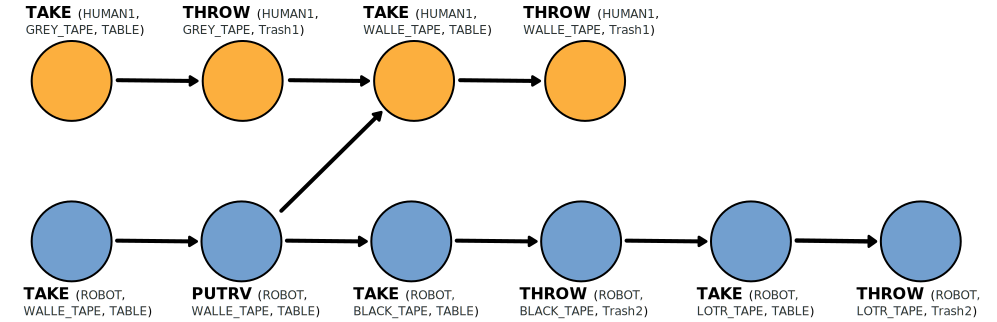
\includegraphics[width=0.8\columnwidth]{integration/hatp_plan2.pdf}
  \caption{A plan with the wasted time social rule}
  \label{plan_hatp2}
\end{figure}

Figure~\ref{plan_hatp2} illustrates an alternative plan to the previous one
(fig.~\ref{plan_hatp1}) if the wasted time social rule is used.  The obtained
shared plan is the best plan according to a global evaluation of these multiple
criteria.

\paragraph{Several levels of cooperation} By tuning its costs and adapting its
social rules, HATP can be used to compute various alternative plans. These
plans can be categorized into several levels of cooperation

\begin{itemize}

    \item helping the human to achieve his goal by acting for him

    \item sharing concrete resources by handing some objects

    \item collaboration of the robot and the human by coordinating their
    actions towards a human-robot joint goal.

\end{itemize}


\subsection{Execution Control}

Depending on experimental setups, the ORO server has been integrated with
several distinct execution controllers. We briefly present them here, with some
details regarding the integration knowledge base/controller.

\paragraph{CSLU Toolkit}
\label{sect|rad}

\begin{figure}
    \centering
    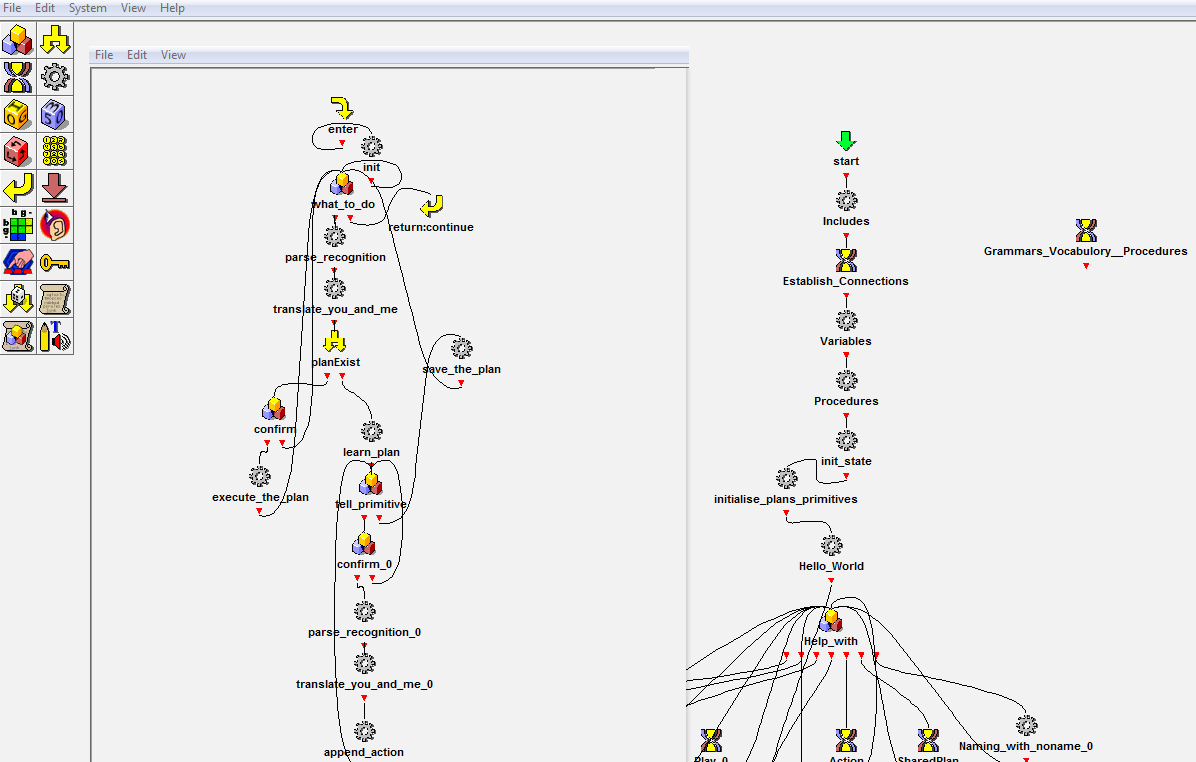
\includegraphics[width=0.4\columnwidth]{integration/rad.png}

    \caption{The CSLU Toolkit allows to program behaviours by building a
    network of connected ``boxes''.}

    \label{fig|rad}
\end{figure}
The CSLU Toolkit is a rapid application development framwork developed at
Oregon University. It comprise of a suite of tools that enable exploration,
learning, and research into speech and human-computer interaction via a user
friendly graphical interface (figure~\ref{fig|rad}). The CSLU toolkit has been
employed in several experiments of the European FP7 CHRIS project (some are
presented at section~\ref{sect|casestudies}, others are presented
in~\cite{Lallee2010, Lallee2011}) to develop scripted verbal interactions with
robots.

The CSLU Toolkit can be easily extended with the TCL scripting language, for
which bindings with the ORO server exist. This enable users to graphically
design interaction experiments that take advantage of the knowledge base and
its reasoning infrastructure to add and retrieve concepts.

\paragraph{CRAM}
\label{sect|cram}

{\sc Cram}~\cite{Beetz2010} (Cognitive Robotic Abstract Machine) is a
RPL-derived framework for rapid development of cognitive robot control programs
that is developed at the Intelligent Autonomous Systems at TU Munich.

{\sc Cram} automatically updates the ORO server whenever an object enters or
leaves the field of view with a perception stack based on the \textsc{CoP}
framework~\cite{Klank2009}.

Therefore, the integration of ORO can be seen as an extension to
the robot's belief state that not only contains abstract identifiers
of the internal object representation used in plans, but also the
semantics and roles of objects in the scenario.

The \emph{Odd One Out} experiment (section~\ref{expe|odd_one_out}) relies on
{\sc Cram} for the robot control.

\paragraph{SHARY}

\paragraph{pyRobots} {\tt pyRobots} is not a real execution controller: it
comprise a set of Python scripts that ease the construction of complex scripted
interaction. {\tt pyRobots} is based on \emph{actions} (high-level tasks like
{\tt goto}, {\tt pick} or {\tt give}\footnote{The complete list, with
documentation, is available online:
\url{http://www.openrobots.org/wiki/wiki/pyrobots}.}) that are combined into
plans.

ORO server is integrated in {\tt pyRobots} via the ORO Python bindings
(presented section~\ref{sect|python-bindings}). The currently performed action
is maintained up-to-date in the server, and actions are free to store or
retreive facts (for instance, the {\tt pick} task add the fact \stmt{myself
hasIn{Right|Left}Hand x}, \concept{x} being replaced by the ID of the object
that is taken.

Events can also be used by the application designer.


\subsection{Integration with natural language processors}

Figure~\ref{fig|dialog-integration} gives a functional overview of the
components involved in the situated dialogue grounding.

\begin{figure}
    \centering
    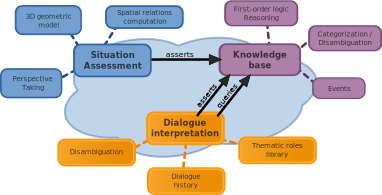
\includegraphics[width=0.7\columnwidth]{integration/dialog_integration.pdf}
    \caption{Schematic view of the integration of a natural language processor
    in the architecture}
    \label{fig|dialog-integration}
\end{figure}

Chapter~\ref{chapter|dialogs} presents in greater details the integration of
the {\sc Dialogs} module for situated natural language processing with ORO.

%%%%%%%%%%%%%%%%%

\section{Towards an Event-Driven, Knowledge-Oriented Architecture}

In this section, we have presented how knowledge streams are organized between
several components: {\it(1)} {\sc ORO}, the ontology-based knowledge server
that stores and maintains classified RDF statements produced by other modules
in agent-specific models and allows information to be retrieved either through
queries or via an event system; {\it(2)} {\sc SPARK}, the grounded,
human-aware, 3D model of the environment that performs all the spatial
reasoning within this architecture, including reasoning involving motion
planing (to compute reachability of objects) and perspective taking, {\it(3)}
{\sc CRAM}, {\sc SHARY}, {\sc pyRobots}, {\sc RAD}, {\sc HATP} as different
examples of execution controllers and symbolic task planners that take
advantage of semantic abstractions provided by knowledge base and {\it(4)} {\sc
Dialogs}, a natural language processor that performs simple grammatical parsing
of English language, grounds the semantic content of the utterance (if
necessary, also interacts with the user to disambiguate), and eventually
generates a RDF representation of the sentence.

Altogether, these components compose an architecture that we call
\emph{knowledge-oriented}:

\begin{itemize} \item{Knowledge is explicitly stored in one central and
consistent repository of facts, accessible by all modules.} \item{Knowledge is
represented in a strict formalism (OWL statements) and with a clearly defined
vocabulary (stated in the {\tt commonsense.oro.owl} ontology).} \item{The first
two points enable both a loosely-coupled architecture where modules can very
easily be removed or replaced by other ones as long as they share the same
semantics (modules are defined by the knowledge they produce),} \item{and a
\emph{symbolic} reactive, event-driven approach to supervision. By managing
events at the same level as the reasoner, we take full advantage of the
inference abilities of ORO to trigger events whose \texttt{true} conditions can
be inferred.} \item{Finally, this architecture allows for the combination of
very different knowledge modalities in a single homogeneous environment,
bringing mutual benefits to components. For instance, the dialogue processing
module can perfectly run without any geometric perception, but its
disambiguation routines can transparently benefit from it when available (since
richer symbolic descriptions of objects are then available).} \end{itemize}

This architecture moves away from standard layered approaches. Interactions
between components are mostly bidirectional and, from the software components
point of view, we do not introduce layers of abstraction (we do, however, have
access to the lower level modules of the robot to execute actions, but all
cognition-related modules reside at the same level). This is especially visible
for the dialogue input processing. This component does not simply act as an
alternative perceptual input to the symbolic database, but also actively
queries previously acquired knowledge to disambiguate and validate the newly
created symbolic knowledge, as we will present in detail in the following
chapter.

Regarding the anchoring question, this architecture is bidirectional. The
components we described provide a \textit{bottom-up} grounding process: SPARK
and \textsc{Dialogs} constantly build and push new symbolic contents about the
world to ORO where it becomes accessible to decisional layers. In parallel, ORO
relies on reasoning in a \textit{top-down} way to produce new facts that may
trigger in return physical behaviours. 

We believe that this \emph{knowledge-oriented} approach has a strong potential
not only to enable rich human-robot interaction, but also as a broader approach
to information alignment and fusion in complex robotic systems.  The
versatility of this paradigm could be illustrated by a simple imaginary
scenario with a blind robot and a deaf robot. The blind robot does not see (no
cameras or alike), but someone can verbally describe a scene to it. On the
other hand, the deaf robot has a good vision system, but cannot process verbal
input.  Without any changes to the software architecture that we described,
supervision modules of both robots would be able to perform equally well (to
actually implement this imaginary situation, the blind robot would of course
need \textit{a priori} 3D models of objects talked about to enable planning or
pick and place actions, and the deaf robot would require at least some gesture
interpretation to understand orders).

This architecture may also contribute to bridge the gap between robotics and
psychology: it provides clear entry points to implement some classical
psychology tests to robots. We presented experiments focused on issues related
to perspective taking. By explicitly enabling independent modeling of the
beliefs of each agent, our architecture is especially well suited to set up
cognitive and psychological experiments (such as the \emph{False-Belief}
experiment), which we plan to further explore.
